\documentclass[12pt,a4paper]{article}

% ─── Encoding ───
\usepackage[utf8]{inputenc}
\usepackage[T1]{fontenc}

% ─── Page layout ───
\usepackage[margin=2.5cm]{geometry}

% ─── Math ───
\usepackage{amsmath,amssymb,amsthm,mathtools}

% ─── Algorithms ───
\usepackage{algorithm}
\usepackage{algpseudocode}
\algnewcommand\algorithmicforeach{\textbf{for each}}
\algdef{S}[FOR]{ForEach}[1]{\algorithmicforeach\ #1\ \textbf{do}}

% ─── TikZ ───
\usepackage{tikz}
\usetikzlibrary{shapes.geometric,arrows.meta,positioning,fit,
                backgrounds,calc,decorations.pathreplacing,matrix}

% ─── Tables ───
\usepackage{booktabs}
\usepackage{tabularx}
\usepackage{multirow}
\usepackage{array}
\usepackage{float}

% ─── Code listings ───
\usepackage{listings}
\usepackage{xcolor}

% ─── Misc ───
\usepackage{caption}
\usepackage{subcaption}
\usepackage{enumitem}
\usepackage{hyperref}
\hypersetup{colorlinks=true,linkcolor=blue!70!black}

% ─── Headers ───
\usepackage{fancyhdr}
\pagestyle{fancy}
\fancyhf{}
\lhead{\footnotesize MIVA-KNIGHT \texttt{domain\_config.py} — Annotated Technical Reference}
\rhead{\footnotesize IT 581 Project}
\cfoot{\thepage}

% ─── Theorem environments ───
\theoremstyle{definition}
\newtheorem{theorem}{Theorem}[section]
\newtheorem{lemma}[theorem]{Lemma}
\newtheorem{definition}[theorem]{Definition}
\newtheorem{axiom}[theorem]{Axiom}
\newtheorem{proposition}[theorem]{Proposition}
\newtheorem{corollary}[theorem]{Corollary}
\theoremstyle{remark}
\newtheorem{remark}[theorem]{Remark}

% ─── Colours ───
\definecolor{cBlue}{RGB}{220,230,245}
\definecolor{cGreen}{RGB}{210,240,210}
\definecolor{cOrange}{RGB}{255,235,215}
\definecolor{cGray}{RGB}{230,230,230}
\definecolor{cPurple}{RGB}{235,220,245}
\definecolor{cTeal}{RGB}{200,235,235}
\definecolor{cYellow}{RGB}{255,248,200}
\definecolor{cDark}{RGB}{40,60,100}
\definecolor{cRed}{RGB}{245,220,220}
\definecolor{cMed}{RGB}{220,245,240}

% ─── Code style ───
\lstset{
  language=Python,
  basicstyle=\ttfamily\small,
  keywordstyle=\color{blue!70!black}\bfseries,
  commentstyle=\color{green!50!black}\itshape,
  stringstyle=\color{orange!70!black},
  numberstyle=\tiny\color{gray},
  frame=single, rulecolor=\color{gray!40},
  numbers=left, breaklines=true,
  tabsize=4, showstringspaces=false,
  morekeywords={dataclass,field,Optional,List,EnvironmentError}
}

% ─── TikZ styles ───
\tikzset{
  basebox/.style={rectangle,rounded corners=4pt,draw=black!60,
                  align=center,font=\footnotesize},
  bluenode/.style={basebox,fill=cBlue,minimum width=3cm,minimum height=0.9cm},
  greennode/.style={basebox,fill=cGreen,minimum width=3cm,minimum height=0.9cm,thick},
  orangenode/.style={basebox,fill=cOrange,minimum width=3cm,minimum height=0.9cm},
  graynode/.style={basebox,fill=cGray,minimum width=3cm,minimum height=0.9cm},
  purplenode/.style={basebox,fill=cPurple,minimum width=3cm,minimum height=0.9cm},
  tealnode/.style={basebox,fill=cTeal,minimum width=3cm,minimum height=0.9cm},
  mednode/.style={basebox,fill=cMed,minimum width=3cm,minimum height=0.9cm,thick},
  warnnode/.style={basebox,fill=cRed,minimum width=3cm,minimum height=0.9cm},
  decnode/.style={diamond,draw=black!70,fill=cYellow,aspect=2.8,
                  align=center,font=\scriptsize},
  arr/.style={->,>=Stealth,thick,color=black!70},
  thkarr/.style={->,>=Stealth,very thick,color=cDark},
  dasharr/.style={->,>=Stealth,dashed,thick,color=gray!70},
  redarr/.style={->,>=Stealth,thick,color=red!60!black},
  grnarr/.style={->,>=Stealth,thick,color=green!50!black}
}

\renewcommand{\algorithmicrequire}{\textbf{Input:}}
\renewcommand{\algorithmicensure}{\textbf{Output:}}

% ──────────────────────────────────────────────
\begin{document}

% ══════════════════════════════════════
%  TITLE PAGE
% ══════════════════════════════════════
\begin{titlepage}
\centering\vspace*{1.5cm}
{\Huge\bfseries\color{cDark} MIVA-KNIGHT}\\[0.4cm]
{\Large\bfseries \texttt{domain\_config.py}}\\[0.3cm]
{\large Annotated Technical Reference}\\[1.0cm]

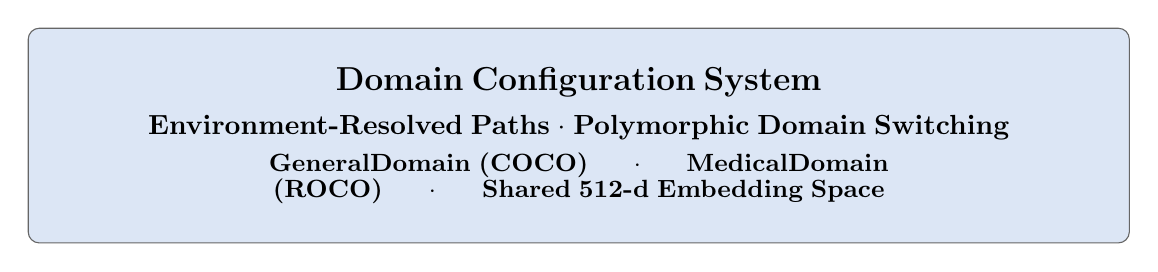
\begin{tikzpicture}
  \node[basebox,fill=cBlue,text width=13cm,inner sep=14pt]{
    \large\bfseries Domain Configuration System\\[4pt]
    \normalsize Environment-Resolved Paths $\cdot$ Polymorphic Domain Switching\\[4pt]
    \small GeneralDomain (COCO) $\;\cdot\;$ MedicalDomain (ROCO) $\;\cdot\;$
    Shared 512-d Embedding Space
  };
\end{tikzpicture}

\vspace{1cm}
{\large\bfseries IT 581 Project}\\[0.3cm]
{\large Oluwakayode Soyinka}\\[0.3cm]
{\normalsize MIVA-KNIGHT: Multimodal Intelligent Voice Assistant — Knight}\\[0.8cm]

\begin{tabular}{ll}
\toprule
\textbf{File}            & \texttt{domain\_config.py} \\
\textbf{Role}            & Runtime domain switching, path resolution, retrieval config \\
\textbf{Sections}        & Module docstring, \texttt{\_root()}, \texttt{\_p()},
                           \texttt{DomainConfig}, \texttt{GeneralDomain},
                           \texttt{MedicalDomain} \\
\textbf{Design Pattern}  & Dataclass inheritance with polymorphic specialisation \\
\textbf{Key Invariant}   & TextProj, AudioProj, BERT, Wav2Vec never swap between domains \\
\bottomrule
\end{tabular}

\vfill
{\small\color{gray}Each code section below is accompanied by formal mathematical
definitions, algorithms, theorems, lemmas, and plain-language explanations,
plus TikZ diagrams wherever a visual aids comprehension.}
\end{titlepage}

\tableofcontents
\newpage

% ══════════════════════════════════════════════════
\section{File Overview and Architecture}
% ══════════════════════════════════════════════════

\subsection{Purpose}

\texttt{domain\_config.py} is the single source of truth for which
files, models, and parameters MIVA-KNIGHT uses when answering a query
in a given domain.
It implements a \emph{polymorphic domain configuration} pattern: all domains
share the same base class (\texttt{DomainConfig}) but override only the
components that differ between domains.

\begin{axiom}[Domain-Agnostic Embedding Space]
The shared 512-dimensional embedding space $\mathbb{S}^{511}$ is
domain-agnostic.  TextProjection, AudioProjection, BERT, and Wav2Vec~2.0
are trained once and used unmodified across all domains.
Only FAISS index, corpus metadata, image encoder weights, knowledge graph,
and NER model change per domain.
This is the central thesis claim: a single contrastive embedding space can
bridge general and medical multimodal retrieval.
\end{axiom}

\subsection{Class Hierarchy}

\begin{figure}[H]
\centering
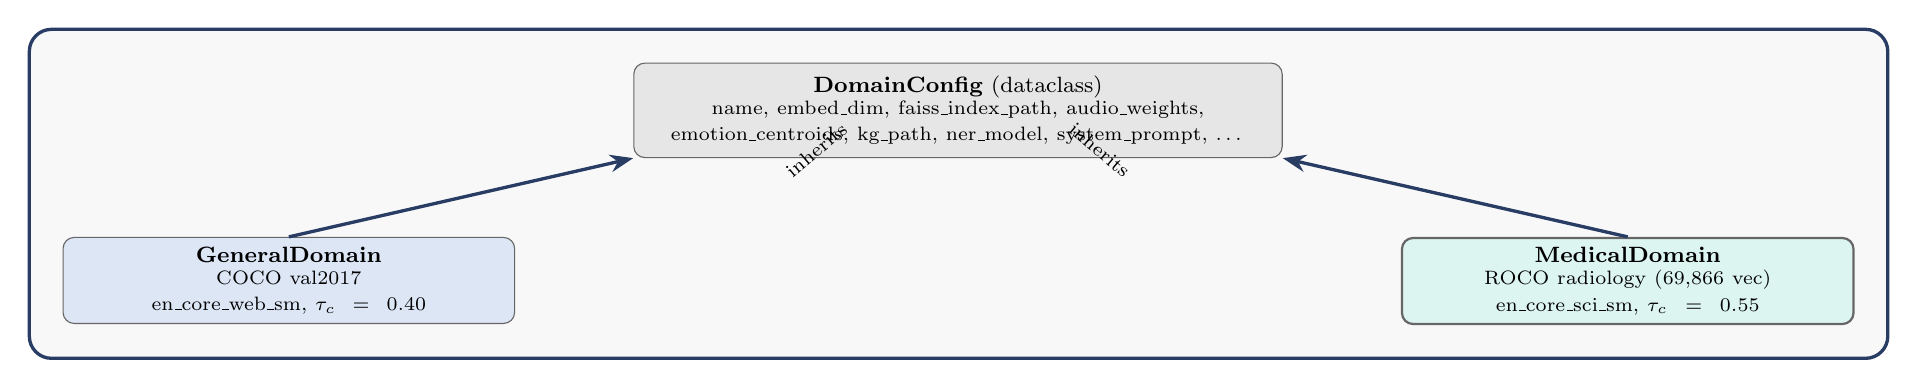
\begin{tikzpicture}[node distance=1.0cm]
  \node[basebox,fill=cGray,text width=8cm,minimum height=1.2cm] (base){
    \textbf{DomainConfig} (dataclass)\\
    \scriptsize name, embed\_dim, faiss\_index\_path, audio\_weights,\\
    \scriptsize emotion\_centroids, kg\_path, ner\_model, system\_prompt, \ldots
  };
  \node[bluenode,text width=5.5cm, below left=1.0cm and 1.5cm of base] (gen){
    \textbf{GeneralDomain}\\
    \scriptsize COCO val2017\\
    \scriptsize en\_core\_web\_sm, $\tau_c=0.40$
  };
  \node[mednode,text width=5.5cm, below right=1.0cm and 1.5cm of base] (med){
    \textbf{MedicalDomain}\\
    \scriptsize ROCO radiology (69,866 vec)\\
    \scriptsize en\_core\_sci\_sm, $\tau_c=0.55$
  };
  \draw[thkarr] (gen.north) -- (base.south west);
  \draw[thkarr] (med.north) -- (base.south east);
  \node[font=\scriptsize,rotate=40] at (-1.8,-0.5) {inherits};
  \node[font=\scriptsize,rotate=-40] at (1.8,-0.5) {inherits};

  \begin{pgfonlayer}{background}
    \node[basebox,fill=cGray!30,very thick,draw=cDark,rounded corners=8pt,
          fit=(base)(gen)(med),inner sep=12pt] {};
  \end{pgfonlayer}
\end{tikzpicture}
\caption{Class hierarchy of \texttt{domain\_config.py}.
\texttt{GeneralDomain} and \texttt{MedicalDomain} both extend \texttt{DomainConfig},
overriding only domain-specific fields.}
\label{fig:class_hierarchy}
\end{figure}

\subsection{Invariant vs Variable Components}

\begin{table}[H]
\centering
\caption{What changes between domains vs what stays constant}
\begin{tabularx}{\textwidth}{lXcc}
\toprule
Component & Description & General & Medical \\
\midrule
\multicolumn{4}{l}{\textit{--- CONSTANT across all domains ---}} \\
TextProjection & BERT $\to$ 512-d projection (Pipeline A) & same & same \\
AudioProjection & Wav2Vec $\to$ 512-d projection (Pipeline C/D) & same & same \\
BERT encoder & Query text encoder & same & same \\
Wav2Vec 2.0 & Audio emotion encoder & same & same \\
\texttt{embed\_dim} & Shared embedding dimension $d=512$ & same & same \\
\midrule
\multicolumn{4}{l}{\textit{--- CHANGES per domain ---}} \\
\texttt{faiss\_index\_path} & FAISS vector index & COCO & ROCO \\
\texttt{corpus\_metadata\_path} & Caption/image metadata & COCO & ROCO \\
\texttt{image\_encoder\_weights} & ImageProjection weights & None & ROCO FT \\
\texttt{finetune\_image\_encoder} & Use fine-tuned image enc & False & True \\
\texttt{kg\_path} & Knowledge graph pickle & general & medical \\
\texttt{ner\_model} & spaCy NER model & \texttt{web\_sm} & \texttt{sci\_sm} \\
\texttt{domain\_entity\_list} & Domain term whitelist & $\emptyset$ & 21 terms \\
\texttt{confidence\_threshold} $\tau_c$ & Retrieval confidence gate & 0.40 & 0.55 \\
\texttt{system\_prompt} & LLM system instruction & general & clinical \\
\bottomrule
\end{tabularx}
\end{table}

% ══════════════════════════════════════════════════
\section{Section 1: Module-Level Imports and Docstring}
% ══════════════════════════════════════════════════

\subsection{Code}

\begin{lstlisting}[caption={Module-level imports and docstring}]
"""
domain_config.py
----------------
MIVA-KNIGHT Domain Configuration

Paths are resolved at instantiation time from the MIVA_PROJECT_ROOT
environment variable, which Cell 2 of the notebook sets automatically:

    os.environ["MIVA_PROJECT_ROOT"] = BASE

This means domain instances always carry absolute paths -- no relative
path issues across Colab sessions, restarts, or machines.
"""

import os
from dataclasses import dataclass, field
from typing import Optional, List
\end{lstlisting}

\subsection{Technical Explanation}

The module imports three standard-library packages:

\begin{enumerate}
  \item \textbf{\texttt{os}} --- operating-system interface, used to read
        environment variables (\texttt{os.environ.get}) and join path segments
        (\texttt{os.path.join}).
  \item \textbf{\texttt{dataclasses}} (\texttt{dataclass}, \texttt{field}) ---
        Python 3.7+ decorator that auto-generates \texttt{\_\_init\_\_},
        \texttt{\_\_repr\_\_}, and \texttt{\_\_eq\_\_} from annotated class attributes,
        eliminating boilerplate configuration object code.
  \item \textbf{\texttt{typing}} (\texttt{Optional}, \texttt{List}) ---
        type annotations for optional strings and string lists, enabling
        static type checking without runtime overhead.
\end{enumerate}

The docstring establishes the \emph{path-resolution contract}: every path
stored in a domain config object is an \emph{absolute} path, derived at
instantiation time from the \texttt{MIVA\_PROJECT\_ROOT} environment variable.

\begin{definition}[Absolute Path Contract]
Let $R = \texttt{MIVA\_PROJECT\_ROOT}$ be the project root directory.
For any relative path fragment $\pi = (p_1, p_2, \ldots, p_k)$, the
corresponding absolute path is:
\[
  \textsc{AbsPath}(\pi) = R \mathbin{/} p_1 \mathbin{/} p_2 \mathbin{/}
  \cdots \mathbin{/} p_k
\]
All \texttt{DomainConfig} path fields satisfy
$\forall f \in F_{\text{path}}: f = \textsc{AbsPath}(\cdot)$
at the time the object is constructed.
\end{definition}

\begin{remark}[Plain-language]
Think of this file as a recipe card for the MIVA-KNIGHT assistant.
The imports at the top are like gathering your kitchen tools before cooking.
The docstring explains the most important rule: every file location written
on the recipe card is a \emph{full address} (``3rd shelf, 2nd drawer, red box''),
never just a local name like ``the red box''.
This prevents the assistant from losing its files when it moves to a new
computer or when Google Colab resets.
\end{remark}

% ══════════════════════════════════════════════════
\section{Section 2: \texttt{\_root()} — Environment Variable Resolver}
% ══════════════════════════════════════════════════

\subsection{Code}

\begin{lstlisting}[caption={\texttt{\_root()} function}]
def _root() -> str:
    root = os.environ.get("MIVA_PROJECT_ROOT", "")
    if not root:
        raise EnvironmentError(
            "MIVA_PROJECT_ROOT is not set.\n"
            "Run Cell 2 in the notebook first, or set manually:\n"
            "  import os; os.environ['MIVA_PROJECT_ROOT'] = '/your/project/path'"
        )
    return root
\end{lstlisting}

\subsection{Flowchart}

\begin{figure}[H]
\centering
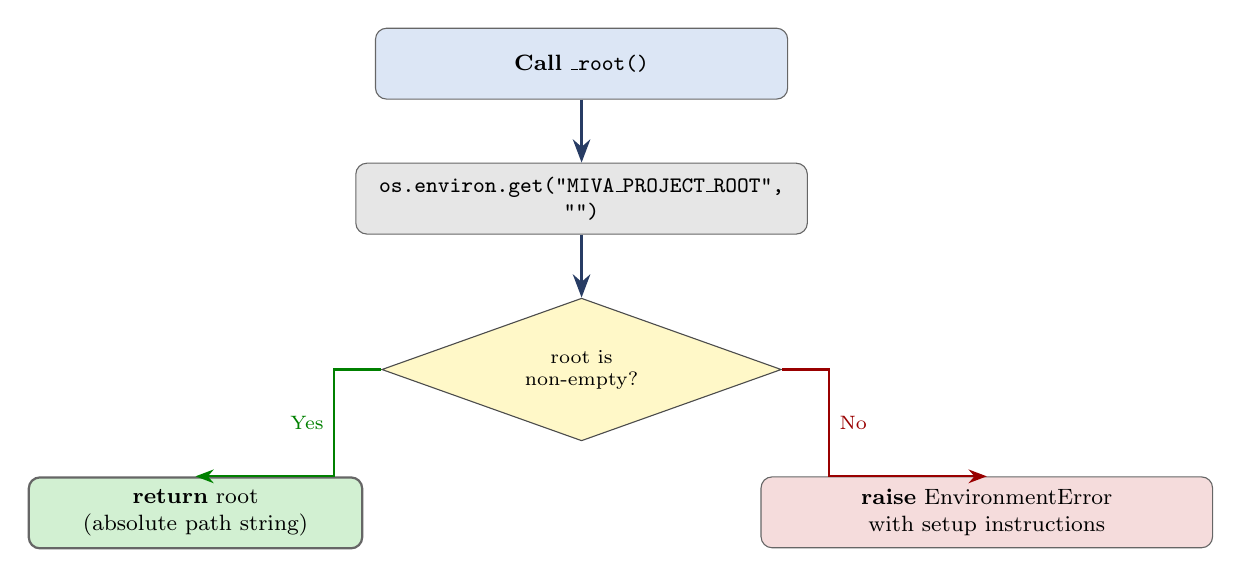
\begin{tikzpicture}[node distance=0.8cm]
  \node[bluenode,text width=5cm] (call)
      {\textbf{Call} \texttt{\_root()}};
  \node[graynode,text width=5.5cm, below=of call] (read)
      {\texttt{os.environ.get("MIVA\_PROJECT\_ROOT", "")}};
  \node[decnode,text width=2.8cm, below=of read] (check)
      {root is\\non-empty?};
  \node[greennode,text width=4cm, below left=0.9cm and 1.5cm of check] (ok)
      {\textbf{return} root\\(absolute path string)};
  \node[warnnode,text width=5.5cm, below right=0.9cm and 1.0cm of check] (err)
      {\textbf{raise} EnvironmentError\\with setup instructions};

  \draw[thkarr] (call) -- (read);
  \draw[thkarr] (read) -- (check);
  \draw[grnarr] (check.west) -- ++(-0.6,0) |- (ok.north)
      node[near start, left, font=\scriptsize]{Yes};
  \draw[redarr] (check.east) -- ++(0.6,0) |- (err.north)
      node[near start, right, font=\scriptsize]{No};
\end{tikzpicture}
\caption{Control flow of \texttt{\_root()}: reads the environment variable
and either returns the root path or raises a descriptive error.}
\label{fig:root_flow}
\end{figure}

\subsection{Technical Explanation}

\begin{definition}[Environment Variable]
An \emph{environment variable} is a key-value pair held in the operating
system's process environment, visible to all code within the same process.
Formally, the environment $\mathcal{E}$ is a partial map
$\mathcal{E}: \text{Key} \rightharpoonup \text{Value}$, and
\[
  \texttt{os.environ.get}(k, d) =
  \begin{cases}
    \mathcal{E}(k) & \text{if } k \in \text{dom}(\mathcal{E}) \\
    d              & \text{otherwise}
  \end{cases}
\]
\end{definition}

\begin{algorithm}[H]
\caption{\texttt{\_root()} — Environment Root Resolution}
\label{alg:root}
\begin{algorithmic}[1]
\Require Environment map $\mathcal{E}$
\Ensure Absolute project root path $R \in \text{String}$, or exception
\State $R \gets \mathcal{E}.\textsc{get}(\texttt{"MIVA\_PROJECT\_ROOT"},\; \texttt{""})$
\If{$R = \texttt{""}$}
  \State \textbf{raise} \texttt{EnvironmentError} with diagnostic message
         \Comment{Fail-fast: never silently return a wrong path}
\EndIf
\State \Return $R$
\end{algorithmic}
\end{algorithm}

\begin{theorem}[Fail-Fast Path Safety]
\texttt{\_root()} implements a \emph{fail-fast} contract: any call to
a \texttt{DomainConfig} constructor before \texttt{MIVA\_PROJECT\_ROOT} is
set raises \texttt{EnvironmentError} with a specific remediation message
rather than silently returning paths containing empty strings.
This prevents the silent creation of paths such as
\texttt{"/indexes/coco\_val2017.faiss"} (with empty root) that would later
cause hard-to-debug \texttt{FileNotFoundError}s at model-load time.
\end{theorem}

\begin{remark}[Plain-language]
Imagine sending a letter with a blank return address.
\texttt{\_root()} is the postal worker who refuses to accept the letter
until you fill in the return address — and helpfully tells you \emph{exactly}
how to do it, rather than just saying ``address invalid''.
The project root is that return address: every other file path in the
system is written relative to it.
\end{remark}

% ══════════════════════════════════════════════════
\section{Section 3: \texttt{\_p()} — Path Builder}
% ══════════════════════════════════════════════════

\subsection{Code}

\begin{lstlisting}[caption={\texttt{\_p()} path builder}]
def _p(*parts: str) -> str:
    """Build an absolute path under the project root."""
    return os.path.join(_root(), *parts)
\end{lstlisting}

\subsection{Technical Explanation}

\begin{definition}[Path Builder Function]
Let $R$ be the project root returned by \texttt{\_root()}, and let
$(p_1, p_2, \ldots, p_k)$ be an ordered tuple of path segments.
The path builder function is:
\[
  \texttt{\_p}(p_1, p_2, \ldots, p_k)
  = R \mathbin{\oplus} p_1 \mathbin{\oplus} p_2 \mathbin{\oplus} \cdots \mathbin{\oplus} p_k
\]
where $\oplus$ denotes the OS-appropriate path separator join
(\texttt{/} on Linux/macOS, \texttt{\textbackslash} on Windows).
\texttt{os.path.join} implements this join in a platform-portable way.
\end{definition}

\begin{algorithm}[H]
\caption{\texttt{\_p()} — Absolute Path Construction}
\label{alg:p}
\begin{algorithmic}[1]
\Require Path segments $p_1, p_2, \ldots, p_k \in \text{String}$
\Ensure Absolute path $P \in \text{String}$
\State $R \gets \textsc{\_root}()$
       \Comment{Raises \texttt{EnvironmentError} if root not set}
\State $P \gets \textsc{os.path.join}(R, p_1, p_2, \ldots, p_k)$
\State \Return $P$
\end{algorithmic}
\end{algorithm}

\subsection{Usage Examples}

\begin{table}[H]
\centering
\caption{Example \texttt{\_p()} calls assuming \texttt{ROOT = "/project"}}
\begin{tabular}{ll}
\toprule
Call & Result \\
\midrule
\texttt{\_p("indexes","coco\_val2017.faiss")} & \texttt{/project/indexes/coco\_val2017.faiss} \\
\texttt{\_p("models","miva\_knight\_pipelineC","audio\_projection.pth")} & \texttt{/project/models/miva\_knight\_pipelineC/audio\_projection.pth} \\
\texttt{\_p("data","roco\_corpus\_metadata.json")} & \texttt{/project/data/roco\_corpus\_metadata.json} \\
\bottomrule
\end{tabular}
\end{table}

\begin{proposition}[Path Portability]
Because \texttt{\_p()} delegates to \texttt{os.path.join}, the resulting
path string is valid on Linux, macOS, and Windows without modification.
Changing \texttt{MIVA\_PROJECT\_ROOT} to any valid root automatically
propagates correct absolute paths to every domain config object in the
process.
\end{proposition}

\begin{remark}[Plain-language]
\texttt{\_p()} is like a GPS that always starts from your current location.
You give it the street address segments (\texttt{"models"}, \texttt{"audio.pth"})
and it prefixes your full home address automatically.
Move to a new city (new machine or Drive folder) and just update the home
address (\texttt{MIVA\_PROJECT\_ROOT}); all directions update themselves.
\end{remark}

% ══════════════════════════════════════════════════
\section{Section 4: \texttt{DomainConfig} — Base Dataclass}
% ══════════════════════════════════════════════════

\subsection{Code}

\begin{lstlisting}[caption={\texttt{DomainConfig} base dataclass}]
@dataclass
class DomainConfig:
    name:                  str            = "base"
    description:           str            = ""
    faiss_index_path:      str            = ""
    corpus_metadata_path:  str            = ""
    embed_dim:             int            = 512
    image_encoder_weights: Optional[str]  = None
    finetune_image_encoder: bool          = False
    audio_weights:         str            = ""
    emotion_centroids:     str            = ""
    kg_path:               str            = ""
    ner_model:             str            = "en_core_web_sm"
    domain_entity_list:    List[str]      = field(default_factory=list)
    dense_top_k:           int            = 20
    rerank_top_n:          int            = 5
    confidence_threshold:  float          = 0.40
    system_prompt:         str            = (...)
\end{lstlisting}

\subsection{Architecture Diagram: DomainConfig Fields by Role}

\begin{figure}[H]
\centering
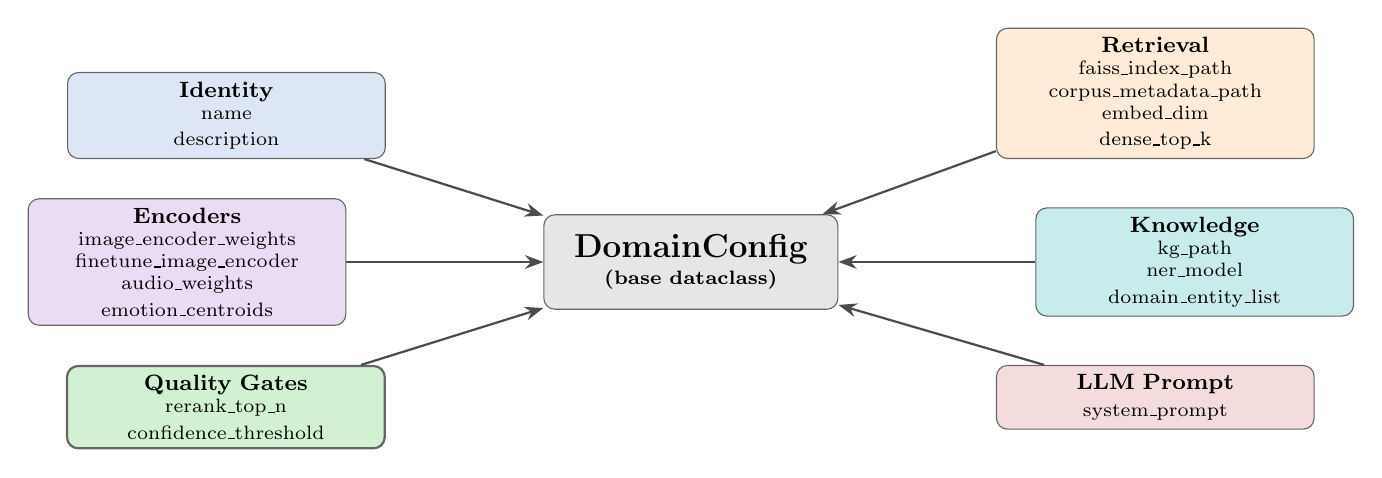
\begin{tikzpicture}[node distance=0.5cm and 0.8cm]

  % Centre: DomainConfig
  \node[basebox,fill=cGray,text width=3.5cm,minimum height=1.2cm] (dc)
      {\large\bfseries DomainConfig\\
       \scriptsize (base dataclass)};

  % Identity group
  \node[bluenode,text width=3.8cm, above left=0.7cm and 2.0cm of dc] (id)
      {\textbf{Identity}\\
       \scriptsize name\\description};

  % Retrieval group
  \node[orangenode,text width=3.8cm, above right=0.7cm and 2.0cm of dc] (ret)
      {\textbf{Retrieval}\\
       \scriptsize faiss\_index\_path\\corpus\_metadata\_path\\embed\_dim\\dense\_top\_k};

  % Encoder group
  \node[purplenode,text width=3.8cm, left=2.5cm of dc] (enc)
      {\textbf{Encoders}\\
       \scriptsize image\_encoder\_weights\\finetune\_image\_encoder\\audio\_weights\\emotion\_centroids};

  % NER/KG group
  \node[tealnode,text width=3.8cm, right=2.5cm of dc] (kg)
      {\textbf{Knowledge}\\
       \scriptsize kg\_path\\ner\_model\\domain\_entity\_list};

  % LLM group
  \node[greennode,text width=3.8cm, below left=0.7cm and 2.0cm of dc] (llm)
      {\textbf{Quality Gates}\\
       \scriptsize rerank\_top\_n\\confidence\_threshold};

  % Prompt group
  \node[basebox,fill=cRed,text width=3.8cm, below right=0.7cm and 2.0cm of dc] (prompt)
      {\textbf{LLM Prompt}\\
       \scriptsize system\_prompt};

  % Arrows
  \foreach \n in {id,ret,enc,kg,llm,prompt}
    \draw[arr] (\n) -- (dc);

\end{tikzpicture}
\caption{\texttt{DomainConfig} field groups by functional role.
All six groups are present in every domain; only the \textit{Encoders},
\textit{Retrieval}, \textit{Knowledge}, \textit{Quality Gates},
and \textit{LLM Prompt} groups differ between \texttt{GeneralDomain}
and \texttt{MedicalDomain}.}
\label{fig:dc_fields}
\end{figure}

\subsection{Technical Explanation}

\begin{definition}[Dataclass]
A Python \emph{dataclass} decorated with \texttt{@dataclass} is a class
whose fields are declared as annotated class-level variables.
The decorator automatically generates:
\begin{enumerate}
  \item \texttt{\_\_init\_\_}: a constructor accepting all fields as keyword arguments with their declared defaults.
  \item \texttt{\_\_repr\_\_}: a developer-readable string representation.
  \item \texttt{\_\_eq\_\_}: structural equality testing field-by-field.
\end{enumerate}
Formally, for a dataclass $D$ with fields
$(f_1 : T_1 = d_1, \ldots, f_n : T_n = d_n)$,
any omitted argument $f_i$ at construction time takes value $d_i$.
\end{definition}

\begin{theorem}[Mutable Default Safety]
The field \texttt{domain\_entity\_list: List[str] = field(default\_factory=list)}
uses \texttt{field(default\_factory=list)} rather than
\texttt{domain\_entity\_list: List[str] = []}
because Python shares a single mutable default object across all instances
when a list literal is used as a default.
Mutations to that list on one instance would silently corrupt all other instances.
\texttt{default\_factory=list} creates a fresh empty list per instance, preventing this.
\end{theorem}

\begin{lemma}[Confidence Threshold Semantics]
The \texttt{confidence\_threshold} $\tau_c \in [0,1]$ acts as a
\emph{quality gate} on FAISS retrieval results.
Let $s_k = \cos(\hat{q}, \hat{d}_k)$ be the cosine similarity of query
$\hat{q}$ to the $k$-th retrieved document $\hat{d}_k$.
The re-ranked candidate set passed to the LLM is:
\[
  \mathcal{C} = \{k \in \{1,\ldots,K\} \mid s_k \geq \tau_c\}
\]
For the general domain $\tau_c = 0.40$; for the medical domain
$\tau_c = 0.55$, reflecting the higher cost of clinical false positives.
\end{lemma}

\subsection{Field-by-Field Reference Table}

\begin{table}[H]
\centering
\caption{\texttt{DomainConfig} field reference}
\begin{tabularx}{\textwidth}{llXl}
\toprule
Field & Type & Purpose & Default \\
\midrule
\texttt{name} & \texttt{str} & Domain identifier string & \texttt{"base"} \\
\texttt{description} & \texttt{str} & Human-readable description & \texttt{""} \\
\texttt{faiss\_index\_path} & \texttt{str} & Path to FAISS binary index & \texttt{""} \\
\texttt{corpus\_metadata\_path} & \texttt{str} & Path to JSON metadata & \texttt{""} \\
\texttt{embed\_dim} & \texttt{int} & Shared embedding dimension $d$ & 512 \\
\texttt{image\_encoder\_weights} & \texttt{Optional[str]} & ImageProjection checkpoint & \texttt{None} \\
\texttt{finetune\_image\_encoder} & \texttt{bool} & Use domain-FT image enc & \texttt{False} \\
\texttt{audio\_weights} & \texttt{str} & AudioProjection checkpoint & \texttt{""} \\
\texttt{emotion\_centroids} & \texttt{str} & Centroid tensor $[C,512]$ & \texttt{""} \\
\texttt{kg\_path} & \texttt{str} & Knowledge graph pickle & \texttt{""} \\
\texttt{ner\_model} & \texttt{str} & spaCy NER model name & \texttt{"en\_core\_web\_sm"} \\
\texttt{domain\_entity\_list} & \texttt{List[str]} & Domain term whitelist & \texttt{[]} \\
\texttt{dense\_top\_k} & \texttt{int} & FAISS ANN candidates $K$ & 20 \\
\texttt{rerank\_top\_n} & \texttt{int} & Top-$N$ after re-rank & 5 \\
\texttt{confidence\_threshold} & \texttt{float} & Cosine similarity gate $\tau_c$ & 0.40 \\
\texttt{system\_prompt} & \texttt{str} & LLM instruction prefix & (base) \\
\bottomrule
\end{tabularx}
\end{table}

\begin{remark}[Plain-language]
\texttt{DomainConfig} is a filled-in form template.
Imagine the assistant has a settings sheet with blank boxes:
``which file cabinet to search?'', ``how strict should the quality check be?'',
``what should the AI say at the start of every answer?''.
The dataclass is that blank form.
\texttt{GeneralDomain} and \texttt{MedicalDomain} are pre-filled versions
of the same form — one for everyday questions, one for medical questions.
\end{remark}

% ══════════════════════════════════════════════════
\section{Section 5: \texttt{GeneralDomain} — COCO Configuration}
% ══════════════════════════════════════════════════

\subsection{Code}

\begin{lstlisting}[caption={\texttt{GeneralDomain} class}]
class GeneralDomain(DomainConfig):
    """
    General domain -- COCO val2017 retrieval backbone.
    Built in Month 1-2. Absolute paths resolved from MIVA_PROJECT_ROOT.
    """
    def __init__(self):
        super().__init__(
            name                  = "general",
            description           = "General-purpose retrieval over COCO natural imagery and captions",
            faiss_index_path      = _p("indexes", "coco_val2017.faiss"),
            corpus_metadata_path  = _p("data", "coco_corpus_metadata.json"),
            image_encoder_weights = None,
            audio_weights         = _p("models", "miva_knight_pipelineC",
                                       "audio_projection.pth"),
            emotion_centroids     = _p("models", "miva_knight_pipelineC",
                                       "emotion_centroids.pt"),
            kg_path               = _p("models", "kg", "ner_kg_general.pkl"),
            ner_model             = "en_core_web_sm",
            dense_top_k           = 20,
            rerank_top_n          = 5,
            confidence_threshold  = 0.40,
            system_prompt         = (
                "You are MIVA-KNIGHT, a helpful multimodal assistant. ..."
            ),
        )
\end{lstlisting}

\subsection{GeneralDomain Architecture Diagram}

\begin{figure}[H]
\centering
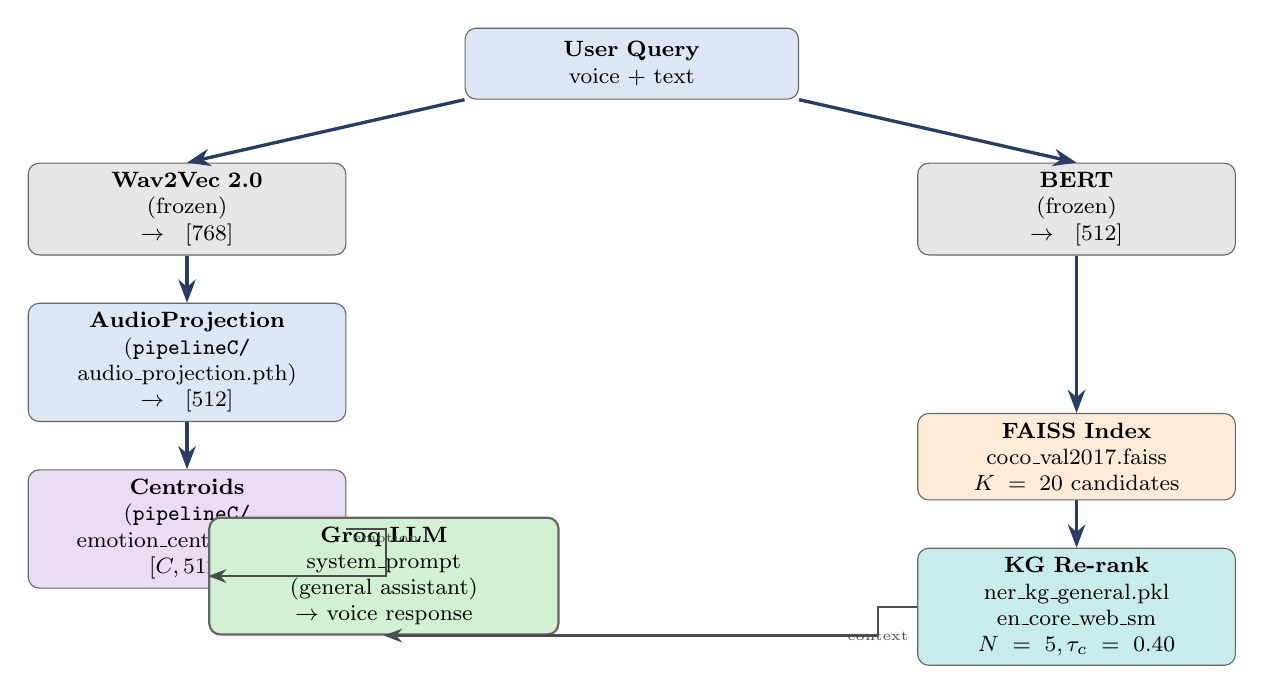
\begin{tikzpicture}[node distance=0.7cm and 1.0cm]

  % Query entry
  \node[bluenode,text width=4cm] (query)
      {\textbf{User Query}\\voice + text};

  % Audio branch
  \node[graynode,text width=3.8cm, below left=0.8cm and 1.5cm of query] (wav)
      {\textbf{Wav2Vec 2.0}\\(frozen)\\$\to [768]$};
  \node[bluenode,text width=3.8cm, below=0.6cm of wav] (aproj)
      {\textbf{AudioProjection}\\(\texttt{pipelineC/}\\audio\_projection.pth)\\$\to [512]$};
  \node[purplenode,text width=3.8cm, below=0.6cm of aproj] (cent)
      {\textbf{Centroids}\\(\texttt{pipelineC/}\\emotion\_centroids.pt)\\$[C, 512]$};

  % Text branch
  \node[graynode,text width=3.8cm, below right=0.8cm and 1.5cm of query] (bert)
      {\textbf{BERT}\\(frozen)\\$\to [512]$};

  % FAISS
  \node[orangenode,text width=3.8cm, below=2.0cm of bert] (faiss)
      {\textbf{FAISS Index}\\coco\_val2017.faiss\\$K=20$ candidates};

  % KG
  \node[tealnode,text width=3.8cm, below=0.6cm of faiss] (kg)
      {\textbf{KG Re-rank}\\ner\_kg\_general.pkl\\en\_core\_web\_sm\\$N=5, \tau_c=0.40$};

  % LLM
  \node[greennode,text width=4.2cm, below=1.2cm of aproj, xshift=2.5cm] (llm)
      {\textbf{Groq LLM}\\system\_prompt\\(general assistant)\\$\to$ voice response};

  \draw[thkarr] (query.south west) -- (wav.north);
  \draw[thkarr] (query.south east) -- (bert.north);
  \draw[thkarr] (wav.south) -- (aproj.north);
  \draw[thkarr] (aproj.south) -- (cent.north);
  \draw[thkarr] (bert.south) -- (faiss.north);
  \draw[thkarr] (faiss.south) -- (kg.north);
  \draw[arr] (cent.east) -- ++(0.5,0) |- (llm.west)
      node[near start,above,font=\tiny]{emotion};
  \draw[arr] (kg.west) -- ++(-0.5,0) |- (llm.south)
      node[near start,below,font=\tiny]{context};

\end{tikzpicture}
\caption{\texttt{GeneralDomain} inference flow. Audio branch detects
emotion via Pipeline C weights; text branch retrieves COCO context via
FAISS and general KG; both feed the LLM with general assistant prompt.}
\label{fig:gen_domain}
\end{figure}

\subsection{Technical Explanation}

\begin{definition}[FAISS Approximate Nearest Neighbour (ANN) Search]
Let $\mathcal{D} = \{\hat{d}_1, \ldots, \hat{d}_N\}$ be the corpus of
$N$ L2-normalised document embeddings in $\mathbb{S}^{511}$ stored in
\texttt{coco\_val2017.faiss}.
Given a query embedding $\hat{q} \in \mathbb{S}^{511}$, FAISS returns
the top-$K$ approximate nearest neighbours by maximum inner product (MIPS):
\[
  \mathcal{R}_K = \arg\text{top-}K_{d \in \mathcal{D}}\; \hat{q} \cdot \hat{d}
  = \arg\text{top-}K_{d \in \mathcal{D}}\; \cos(\hat{q}, \hat{d})
\]
For \texttt{GeneralDomain}: $K = \texttt{dense\_top\_k} = 20$,
$N_{\text{COCO}} \approx 118{,}287$ images.
\end{definition}

\begin{algorithm}[H]
\caption{\texttt{GeneralDomain} Instantiation}
\label{alg:gen_init}
\begin{algorithmic}[1]
\Require \texttt{MIVA\_PROJECT\_ROOT} is set in the environment
\Ensure A \texttt{GeneralDomain} object with all absolute paths populated
\State Verify \texttt{\_root()} returns non-empty $R$
\State \textbf{Fields set at construction:}
\State $\quad\texttt{faiss\_index\_path} \gets R\,/\,\texttt{indexes}\,/\,\texttt{coco\_val2017.faiss}$
\State $\quad\texttt{corpus\_metadata\_path} \gets R\,/\,\texttt{data}\,/\,\texttt{coco\_corpus\_metadata.json}$
\State $\quad\texttt{image\_encoder\_weights} \gets \textbf{None}$ \Comment{Base Pipeline A weights, no domain FT}
\State $\quad\texttt{audio\_weights} \gets R\,/\,\texttt{models}\,/\,\texttt{pipelineC}\,/\,\texttt{audio\_projection.pth}$
\State $\quad\texttt{emotion\_centroids} \gets R\,/\,\texttt{models}\,/\,\texttt{pipelineC}\,/\,\texttt{emotion\_centroids.pt}$
\State $\quad\texttt{kg\_path} \gets R\,/\,\texttt{models}\,/\,\texttt{kg}\,/\,\texttt{ner\_kg\_general.pkl}$
\State $\quad\texttt{ner\_model} \gets \texttt{"en\_core\_web\_sm"}$
\State $\quad\texttt{dense\_top\_k} \gets 20$, $\texttt{rerank\_top\_n} \gets 5$
\State $\quad\texttt{confidence\_threshold} \gets 0.40$
\State \Return fully initialised \texttt{GeneralDomain} object
\end{algorithmic}
\end{algorithm}

\begin{lemma}[Null Image Encoder in GeneralDomain]
\texttt{image\_encoder\_weights = None} in \texttt{GeneralDomain}
indicates that the pipeline uses the \emph{base} ImageProjection weights
trained during Pipeline A (Month~1--2) on COCO, rather than any
domain-fine-tuned variant.
The pipeline code checks:
\[
  \texttt{finetune\_image\_encoder} = \texttt{False}
  \implies \text{load base ImageProjection weights}
\]
This is both correct (COCO ImageProjection \emph{is} the general domain
encoder) and space-efficient (no duplicate checkpoint path required).
\end{lemma}

\begin{proposition}[Confidence Threshold 0.40 for General Domain]
A confidence threshold of $\tau_c = 0.40$ is appropriate for
general-domain (COCO) retrieval because:
\begin{enumerate}
  \item COCO captions are diverse and often loosely related to the query.
  \item False negatives (rejecting a relevant result) are more costly
        than false positives (including a weakly relevant result) for
        general-knowledge queries.
  \item A lower threshold maximises recall at the cost of some precision,
        which the LLM can handle by discarding off-topic context.
\end{enumerate}
\end{proposition}

\begin{remark}[Plain-language]
\texttt{GeneralDomain} is the ``everyday mode'' of the MIVA-KNIGHT assistant.
Imagine a smart librarian who searches a general-purpose encyclopaedia (COCO),
uses standard English language tools to find named entities, and applies a
moderately lenient quality check (40\%) before passing answers to the LLM.
The audio emotion detector still uses Pipeline C weights regardless of domain —
the assistant's ability to hear \emph{how} you feel never changes, only
\emph{what it searches} for answers.
\end{remark}

% ══════════════════════════════════════════════════
\section{Section 6: \texttt{MedicalDomain} — ROCO Configuration}
% ══════════════════════════════════════════════════

\subsection{Code}

\begin{lstlisting}[caption={\texttt{MedicalDomain} class}]
class MedicalDomain(DomainConfig):
    def __init__(self):
        super().__init__(
            name                  = "medical",
            faiss_index_path      = _p("indexes", "roco_medical.faiss"),
            corpus_metadata_path  = _p("data", "roco_corpus_metadata.json"),
            image_encoder_weights = _p("models", "miva_knight_month4",
                                       "image_projection_roco.pth"),
            finetune_image_encoder = True,
            audio_weights         = _p("models", "miva_knight_pipelineC",
                                       "audio_projection.pth"),   # UNCHANGED
            emotion_centroids     = _p("models", "miva_knight_pipelineC",
                                       "emotion_centroids.pt"),   # UNCHANGED
            kg_path               = _p("models", "kg", "ner_kg_medical.pkl"),
            ner_model             = "en_core_sci_sm",
            domain_entity_list    = [
                "pneumonia", "effusion", "atelectasis", "cardiomegaly",
                "consolidation", "infiltrate", "opacity", "bilateral",
                "pleural", "nodule", "mass", "fracture", "edema",
                "pneumothorax", "fibrosis", "emphysema", "trachea",
                "mediastinum", "diaphragm", "hilum", "costophrenic",
            ],
            dense_top_k           = 20,
            rerank_top_n          = 5,
            confidence_threshold  = 0.55,
            system_prompt         = (
                "You are MIVA-KNIGHT, a clinical information assistant. ..."
            ),
        )
\end{lstlisting}

\subsection{MedicalDomain Architecture Diagram}

\begin{figure}[H]
\centering
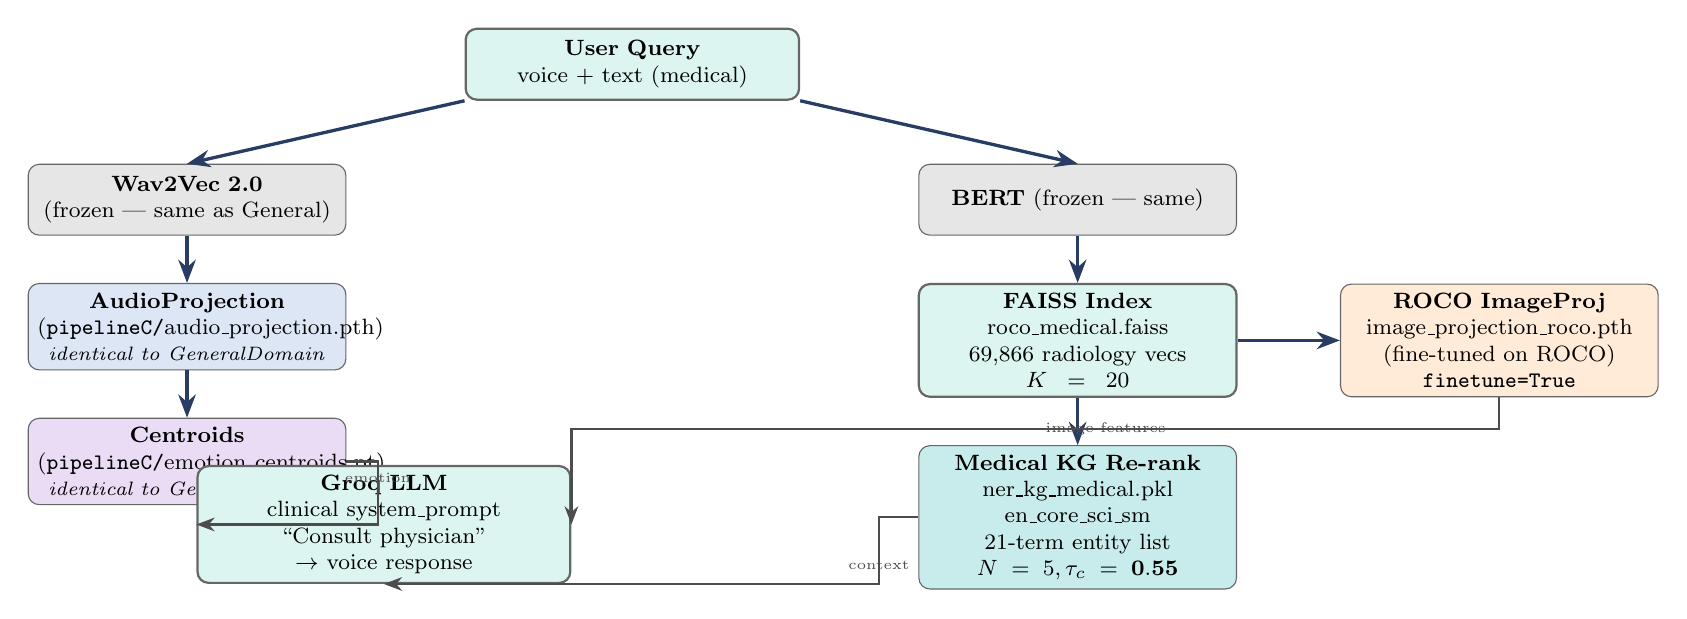
\begin{tikzpicture}[node distance=0.7cm and 1.0cm]

  \node[mednode,text width=4cm] (query)
      {\textbf{User Query}\\voice + text (medical)};

  % Audio --- identical to GeneralDomain
  \node[graynode,text width=3.8cm, below left=0.8cm and 1.5cm of query] (wav)
      {\textbf{Wav2Vec 2.0}\\(frozen — same as General)};
  \node[bluenode,text width=3.8cm, below=0.6cm of wav] (aproj)
      {\textbf{AudioProjection}\\(\texttt{pipelineC/}audio\_projection.pth)\\
       \scriptsize\textit{identical to GeneralDomain}};
  \node[purplenode,text width=3.8cm, below=0.6cm of aproj] (cent)
      {\textbf{Centroids}\\(\texttt{pipelineC/}emotion\_centroids.pt)\\
       \scriptsize\textit{identical to GeneralDomain}};

  % Text branch
  \node[graynode,text width=3.8cm, below right=0.8cm and 1.5cm of query] (bert)
      {\textbf{BERT} (frozen — same)};

  % ROCO FAISS
  \node[mednode,text width=3.8cm, below=0.6cm of bert] (faiss)
      {\textbf{FAISS Index}\\roco\_medical.faiss\\69,866 radiology vecs\\$K=20$};

  % Medical KG + NER
  \node[tealnode,text width=3.8cm, below=0.6cm of faiss] (kg)
      {\textbf{Medical KG Re-rank}\\ner\_kg\_medical.pkl\\en\_core\_sci\_sm\\
       21-term entity list\\$N=5, \tau_c=\mathbf{0.55}$};

  % Image encoder
  \node[basebox,fill=cOrange,text width=3.8cm, right=1.3cm of faiss] (imgenc)
      {\textbf{ROCO ImageProj}\\image\_projection\_roco.pth\\(fine-tuned on ROCO)\\
       \texttt{finetune=True}};

  % LLM
  \node[mednode,text width=4.5cm, below=1.2cm of aproj, xshift=2.5cm] (llm)
      {\textbf{Groq LLM}\\clinical system\_prompt\\``Consult physician''\\
       $\to$ voice response};

  \draw[thkarr] (query.south west) -- (wav.north);
  \draw[thkarr] (query.south east) -- (bert.north);
  \draw[thkarr] (wav.south) -- (aproj.north);
  \draw[thkarr] (aproj.south) -- (cent.north);
  \draw[thkarr] (bert.south) -- (faiss.north);
  \draw[thkarr] (faiss.south) -- (kg.north);
  \draw[thkarr] (faiss.east) -- (imgenc.west);
  \draw[arr] (cent.east) -- ++(0.4,0) |- (llm.west)
      node[near start,above,font=\tiny]{emotion};
  \draw[arr] (kg.west) -- ++(-0.5,0) |- (llm.south)
      node[near start,below,font=\tiny]{context};
  \draw[arr] (imgenc.south) -- ++(0,-0.4) -| (llm.east)
      node[near start,right,font=\tiny]{image features};

\end{tikzpicture}
\caption{\texttt{MedicalDomain} inference flow. The audio branch (emotion detection)
is \textit{identical} to \texttt{GeneralDomain}. The text/image retrieval branch
switches to the ROCO FAISS index, ROCO-fine-tuned ImageProjection, medical KG,
and scispaCy NER, with a stricter confidence gate of 0.55.}
\label{fig:med_domain}
\end{figure}

\subsection{Technical Explanation}

\begin{theorem}[Domain-Agnostic Embedding Space]
\label{thm:da}
Let $\phi_T: \text{Text} \to \mathbb{S}^{511}$ be the TextProjection and
$\phi_A: \text{Audio} \to \mathbb{S}^{511}$ be the AudioProjection.
Both are trained on contrastive objectives that are \emph{label-free}
with respect to domain (InfoNCE on COCO; SupCon on RAVDESS/CREMA-D).
They therefore map inputs from any domain to the same metric space.
The \texttt{MedicalDomain} uses \emph{the same} $\phi_A$ and $\phi_T$
(same checkpoint paths as \texttt{GeneralDomain}), demonstrating that:
\[
  \phi_A^{\text{General}} = \phi_A^{\text{Medical}}
  \quad\text{and}\quad
  \phi_T^{\text{General}} = \phi_T^{\text{Medical}}
\]
Only the corpus-specific components (FAISS, KG, image encoder) change.
\end{theorem}

\begin{definition}[ROCO Medical FAISS Index]
\texttt{roco\_medical.faiss} contains $N_{\text{ROCO}} = 69{,}866$
L2-normalised image-caption embedding vectors from the ROCO radiology
dataset, built using the ROCO fine-tuned ImageProjection
\texttt{image\_projection\_roco.pth}.
FAISS MIPS retrieval on this index returns:
\[
  \mathcal{R}_{20} = \arg\text{top-}20_{d \in \mathcal{D}_{\text{ROCO}}}\;
  \hat{q} \cdot \hat{d}
\]
\end{definition}

\begin{algorithm}[H]
\caption{Domain Entity NER Filtering (Medical Domain)}
\label{alg:ner_filter}
\begin{algorithmic}[1]
\Require Query text $q$, NER model $\mathcal{M} = \texttt{en\_core\_sci\_sm}$,
         entity whitelist $\mathcal{W}$ (21 radiology terms)
\Ensure Boolean: query contains at least one medical entity
\State $\textit{doc} \gets \mathcal{M}(q)$ \Comment{scispaCy parse}
\State $E \gets \{\textit{ent.text.lower}() \mid \textit{ent} \in \textit{doc}.\textit{ents}\}$
       \Comment{Extracted named entities}
\State $M \gets E \cap \mathcal{W}$ \Comment{Intersection with whitelist}
\If{$M \neq \emptyset$}
  \State \Return \textbf{True} \Comment{Route query to MedicalDomain}
\Else
  \State \Return \textbf{False} \Comment{Route to GeneralDomain}
\EndIf
\end{algorithmic}
\end{algorithm}

\begin{lemma}[Stricter Confidence Gate for Clinical Safety]
\label{lem:conf}
For medical retrieval, $\tau_c = 0.55 > 0.40$ (general domain) because:
let $\text{FP}$ denote a false-positive retrieval (incorrect medical
fact passed to the LLM) and $\text{FN}$ a false-negative (correct fact
withheld).
In clinical information contexts, $\text{cost}(\text{FP}) \gg \text{cost}(\text{FN})$
because a mis-stated medical fact could mislead a patient.
Raising $\tau_c$ reduces $\text{FP}$ at the cost of increased $\text{FN}$,
trading completeness for safety.
The system prompt compensates for $\text{FN}$ by explicitly instructing
the LLM to acknowledge insufficient context.
\end{lemma}

\subsection{Medical Entity Whitelist}

The 21-term \texttt{domain\_entity\_list} covers the most frequent
radiology findings in the ROCO dataset:

\begin{table}[H]
\centering
\caption{MedicalDomain entity whitelist — 21 radiology terms}
\begin{tabular}{lll}
\toprule
Pulmonary & Cardiac & Structural \\
\midrule
pneumonia & cardiomegaly & trachea \\
effusion & & mediastinum \\
atelectasis & & diaphragm \\
consolidation & & hilum \\
infiltrate & & costophrenic \\
opacity & & fracture \\
pleural & & \\
nodule & & \\
mass & & \\
edema & & \\
pneumothorax & & \\
fibrosis & & \\
emphysema & & \\
bilateral & & \\
\bottomrule
\end{tabular}
\end{table}

\begin{remark}[Plain-language]
\texttt{MedicalDomain} is the ``clinical mode'' of the assistant.
Think of it as switching the librarian's reference section from a general
encyclopaedia to a radiology textbook library (ROCO, 69,866 medical images).
The librarian's hearing aids (emotion detection) don't change —
the assistant still detects if you sound frightened or confused.
But the quality bar for what counts as a good answer goes up
(from 40\% to 55\% similarity), and every answer now ends with
``consult a physician'', because medical misinformation is more
dangerous than general misinformation.
The medical librarian also has a special medical dictionary (scispaCy +
RadLex) to better recognise clinical terms like ``bilateral consolidation''
or ``pneumothorax''.
\end{remark}

% ══════════════════════════════════════════════════
\section{Domain Switching Flowchart}
% ══════════════════════════════════════════════════

\begin{figure}[H]
\centering
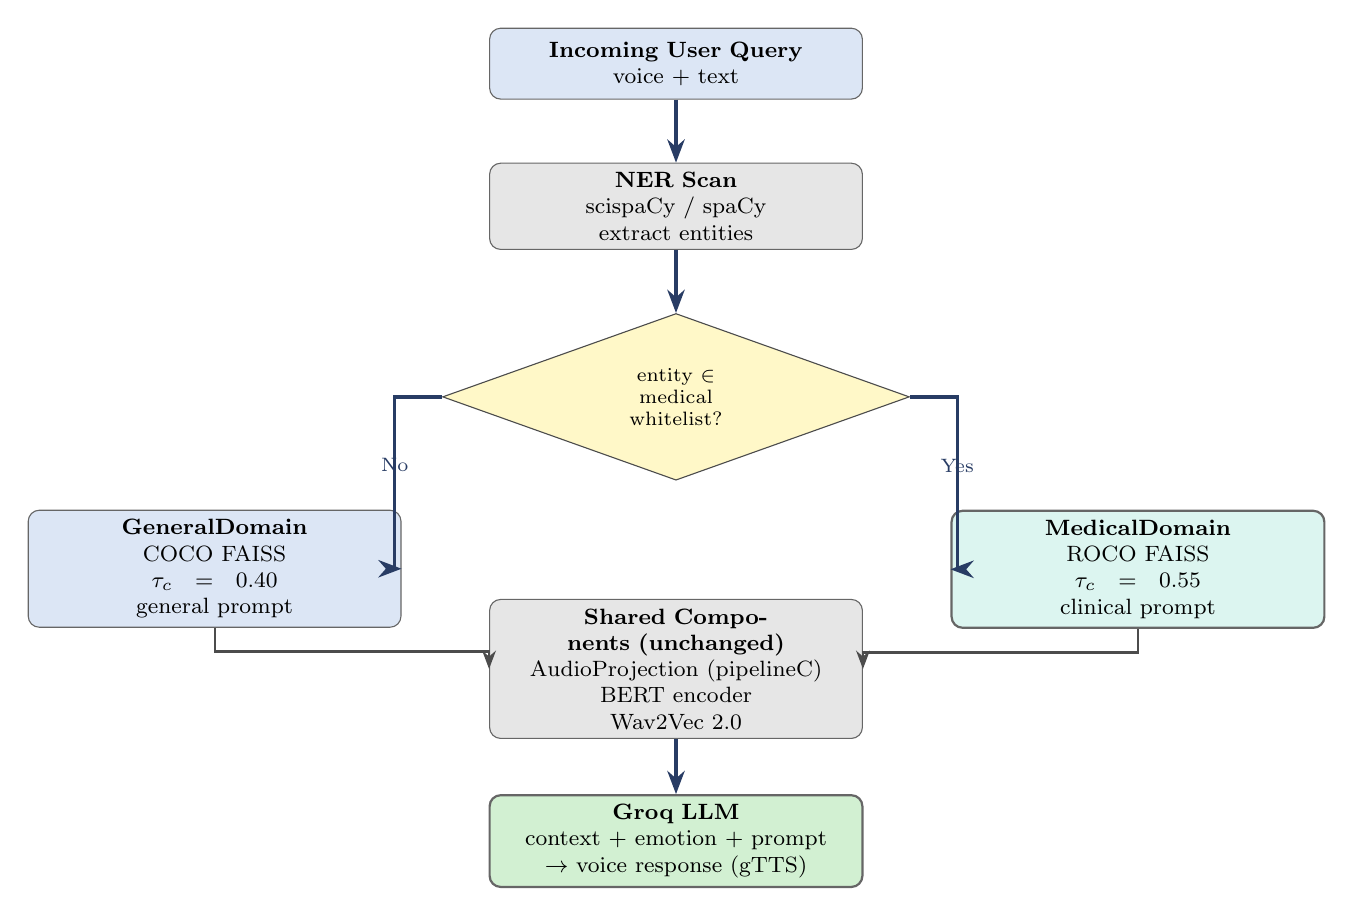
\begin{tikzpicture}[node distance=0.8cm and 1.2cm]

  \node[bluenode,text width=4.5cm] (query)
      {\textbf{Incoming User Query}\\voice + text};

  \node[graynode,text width=4.5cm, below=of query] (ner)
      {\textbf{NER Scan}\\scispaCy / spaCy\\extract entities};

  \node[decnode,text width=3.0cm, below=of ner] (dec)
      {entity $\in$\\medical\\whitelist?};

  \node[mednode,text width=4.5cm, below right=0.9cm and 2.0cm of dec] (meddomain)
      {\textbf{MedicalDomain}\\ROCO FAISS\\$\tau_c = 0.55$\\clinical prompt};

  \node[bluenode,text width=4.5cm, below left=0.9cm and 2.0cm of dec] (gendomain)
      {\textbf{GeneralDomain}\\COCO FAISS\\$\tau_c = 0.40$\\general prompt};

  \node[graynode,text width=4.5cm, below=1.5cm of dec] (shared)
      {\textbf{Shared Components (unchanged)}\\AudioProjection (pipelineC)\\
       BERT encoder\\Wav2Vec 2.0};

  \node[greennode,text width=4.5cm, below=0.7cm of shared] (llm)
      {\textbf{Groq LLM}\\context + emotion + prompt\\$\to$ voice response (gTTS)};

  \draw[thkarr] (query) -- (ner);
  \draw[thkarr] (ner) -- (dec);
  \draw[thkarr] (dec.east) -- ++(0.6,0) |- (meddomain.west)
      node[near start, above, font=\scriptsize]{Yes};
  \draw[thkarr] (dec.west) -- ++(-0.6,0) |- (gendomain.east)
      node[near start, above, font=\scriptsize]{No};
  \draw[arr] (meddomain.south) -- ++(0,-0.3) -| (shared.east);
  \draw[arr] (gendomain.south) -- ++(0,-0.3) -| (shared.west);
  \draw[thkarr] (shared) -- (llm);

\end{tikzpicture}
\caption{Domain switching logic. A single NER scan routes the query to either
\texttt{GeneralDomain} or \texttt{MedicalDomain}. The shared audio/text encoders
are never swapped; only the retrieval stack changes.}
\label{fig:domain_switch}
\end{figure}

% ══════════════════════════════════════════════════
\section{Theoretical Summary}
% ══════════════════════════════════════════════════

\subsection{Key Formal Results}

\begin{theorem}[Polymorphic Domain Configuration Correctness]
Let $\mathcal{D}_G = \texttt{GeneralDomain()}$ and
$\mathcal{D}_M = \texttt{MedicalDomain()}$.
By construction (both call \texttt{super().\_\_init\_\_} with shared
\texttt{audio\_weights} and \texttt{emotion\_centroids} pointing to
Pipeline~C checkpoints):
\[
  \mathcal{D}_G.\texttt{audio\_weights} = \mathcal{D}_M.\texttt{audio\_weights}
\]
\[
  \mathcal{D}_G.\texttt{emotion\_centroids} = \mathcal{D}_M.\texttt{emotion\_centroids}
\]
Therefore the emotion detection sub-system
$\phi_A \circ \textsc{ArgmaxCentroid}$ is \emph{identical} in both domains,
satisfying the domain-agnostic embedding space axiom.
\end{theorem}

\begin{corollary}[Single Emotion Model for All Domains]
Adding a new domain $\mathcal{D}_X$ (e.g., LegalDomain, EducationDomain)
requires only: (1) a domain FAISS index, (2) corpus metadata JSON,
(3) a domain knowledge graph, and (4) an appropriate NER model and entity
list. The AudioProjection, emotion centroids, BERT, and Wav2Vec~2.0 are
reused without modification.
\end{corollary}

\begin{theorem}[Path Resolution Correctness]
For any domain $\mathcal{D}$ instantiated after setting
\texttt{MIVA\_PROJECT\_ROOT} $= R$,
all path fields $f \in F_{\text{path}}(\mathcal{D})$ satisfy:
\[
  f = R \mathbin{/} \pi_f
\]
for the corresponding relative path fragment $\pi_f$.
This is guaranteed by \texttt{\_p()} calling \texttt{\_root()} at
\emph{instantiation time} (not at import time), so the environment
variable is always read from the current process state.
\end{theorem}

\begin{lemma}[Retrieval Pipeline Parameters]
The two-stage retrieval pipeline for any domain $\mathcal{D}$ operates as:
\begin{enumerate}
  \item \textbf{Dense retrieval}: FAISS ANN returns top-$K$ candidates
        where $K = \mathcal{D}.\texttt{dense\_top\_k} = 20$.
  \item \textbf{Re-ranking}: KG entity overlap and cosine similarity
        filter to top-$N$ where $N = \mathcal{D}.\texttt{rerank\_top\_n} = 5$.
  \item \textbf{Confidence gate}: Only candidates with
        $s_k \geq \mathcal{D}.\texttt{confidence\_threshold}$ are passed
        to the LLM.
\end{enumerate}
The final candidate set $\mathcal{C}^* \subseteq \{1,\ldots,N\}$ satisfies:
\[
  |\mathcal{C}^*| \leq N = 5, \quad
  \forall k \in \mathcal{C}^*: s_k \geq \tau_c
\]
\end{lemma}

% ══════════════════════════════════════════════════
\section{Complete Domain Comparison Reference}
% ══════════════════════════════════════════════════

\begin{table}[H]
\centering
\caption{Complete side-by-side comparison: \texttt{GeneralDomain} vs \texttt{MedicalDomain}}
\begin{tabularx}{\textwidth}{lXX}
\toprule
Field & \texttt{GeneralDomain} & \texttt{MedicalDomain} \\
\midrule
\texttt{name} & \texttt{"general"} & \texttt{"medical"} \\
\texttt{faiss\_index\_path} & \texttt{indexes/coco\_val2017.faiss} & \texttt{indexes/roco\_medical.faiss} \\
\texttt{corpus\_metadata\_path} & \texttt{data/coco\_corpus\_metadata.json} & \texttt{data/roco\_corpus\_metadata.json} \\
\texttt{image\_encoder\_weights} & \texttt{None} (base Pipeline A) & \texttt{models/month4/image\_projection\_roco.pth} \\
\texttt{finetune\_image\_encoder} & \texttt{False} & \texttt{True} \\
\texttt{audio\_weights} & \texttt{models/pipelineC/audio\_projection.pth} & \textbf{same} \\
\texttt{emotion\_centroids} & \texttt{models/pipelineC/emotion\_centroids.pt} & \textbf{same} \\
\texttt{kg\_path} & \texttt{models/kg/ner\_kg\_general.pkl} & \texttt{models/kg/ner\_kg\_medical.pkl} \\
\texttt{ner\_model} & \texttt{en\_core\_web\_sm} & \texttt{en\_core\_sci\_sm} \\
\texttt{domain\_entity\_list} & \texttt{[]} & 21 radiology terms \\
\texttt{dense\_top\_k} & 20 & 20 \\
\texttt{rerank\_top\_n} & 5 & 5 \\
\texttt{confidence\_threshold} $\tau_c$ & 0.40 & \textbf{0.55} \\
\texttt{system\_prompt} & General assistant & Clinical with disclaimer \\
\bottomrule
\end{tabularx}
\end{table}

\begin{remark}[Plain-language summary of the whole file]
This entire file does one elegant thing: it provides two ``mode settings''
for the MIVA-KNIGHT assistant — general mode and medical mode.
\begin{description}[leftmargin=1.5cm]
  \item[\texttt{\_root()}] is the safety guard that makes sure you've told
    the program where your project lives before it tries to find any files.
  \item[\texttt{\_p()}] is the address builder that takes a short relative
    path like \texttt{"models/audio.pth"} and turns it into a full computer
    address.
  \item[\texttt{DomainConfig}] is the blank settings form with sensible
    default values for every field.
  \item[\texttt{GeneralDomain}] fills in the form for answering everyday questions,
    using the COCO image-caption database.
  \item[\texttt{MedicalDomain}] fills in the form for answering medical questions,
    using the ROCO radiology database, with stricter quality checks and
    a disclaimer on every answer.
\end{description}
The key insight is that the voice emotion detector never changes mode —
the same trained model listens to how you sound whether you're asking
about cooking or a chest X-ray.
Only the knowledge library and quality threshold switch.
\end{remark}

\end{document}
